\chapter{Variational quantum algorithms} 
\label{chap:vqas}

% What do we want to say?
% We want to explain VQE and PEA.


As we mentioned earlier, present-day quantum computers are a long way from cracking encryption. Nonetheless, there are efforts to find use for quantum computers in the NISQ era. An important line of research is the research of variational quantum algorithms (VQAs). These algorithms rely on a feedback loop between the quantum device and the classical computer. Most often, the quantum device evaluates some kind of cost function (or its gradient), while the classical device performs optimization using the data from the quantum device. In this chapter we focus on this approach to quantum computation. This chapter is mostly devoted to variational quantum eigensolver, however, many ideas are applicable for any variational quantum algorithm.


% \todo{Optimization problems are all around us.
% There are continuous problems (e.g.~linear programming, some airfoil stuff, some other nice examples), and there are discrete problems.
% Both are difficult.
% Here we describe some attempts at embedding optimization tasks}


\section{Variational principle}

Consider a Hermitian operator $H$. We do not know its spectrum, but we have some kind of guess about its ground state $\ket{\psi_{\text{guess}}}$. We know that the guess is not the true state, but we hope that some variation of this guess is close to the truth. So, we can introduce some family of the states $\ket{\psi(\theta)}$. Now, since any state is a linear combination of the ground state and excited states, the energy of that state is never below the ground state energy:

\begin{equation}
    \label{eq:variational_principle}
    E(\theta) = \frac{\bra{\psi(\theta)} H \ket{\psi(\theta)}}
         {\braket{\psi(\theta)}{\psi(\theta)}} \geq E_{gs}.
\end{equation}

This means that if we pick $\theta$ so that $E(\theta)$ is minimal, we can find a state that is the best approximation of the ground state in the sense of energy.

% \begin{example}
%     Consider a Hamiltonian of a harmonic oscillator...
% \end{example}

\subsection{Toy example: spin model}
% \textbf{For parallelism, it may make sense to also explain the PEA here.}
% What do we want from a toy example?
% It should be accessible to a layman.
% We know that it's kind of difficult.
% I want to describe the TFIM model for two qubits.
% Should we solve this model exactly?
% Should there be a numerical section here too?
% This section can be an example for the variational principle: just make an ansatz as a linear combination of |00> and |++>
% Don't forget to include that for this toy example, there is an exact solution.
% The difficulty for a layman is to understand that the target Hamiltonian is abstracted away into the set of instructions on how to measure the states.
% Perhaps there should be a whole section on how to measure variables.

Consider the following Hamiltonian describing two interacting spins in an external magnetic field:

\begin{equation}
    \label{eq:tfim_simple}
    H = J Z \otimes Z + h(X \otimes \id + \id \otimes X) \equiv J Z_1 Z_2 + h(X_1 + X_2).
\end{equation}

For $h = 0, J<0$, the ground state space of this system is obviously spanned by two product states: $\ket{00}$ and $\ket{11}$. 
For $J = 0, h>0$, the unique ground state is a product state $\ket{++} \equiv \frac{1}{2} (\ket{0} + \ket{1}) \otimes (\ket{0} + \ket{1})$. 
For generic values of $J$ and $h$, the ground state is not necessarily a product state. 
Intuitively, the reason is that the two terms in the Hamiltonian compete with each other, and neither of the product states is a good solution.
What if there are $n$ spins in the magnetic field? The Hamiltonian of this model (the \textit{transverse field Ising model}, TFI) is then as follows:

\begin{equation}
    \label{eq:tfim_toy}
    H = J \sum_{i=1}^{n-1} Z_i Z_{i+1} + h \sum_{i=1}^n X_i.
\end{equation}

The same reasoning still applies. In the limiting cases, there are simple product ground states, while generic case is more complicated. In fact, the case $J=h$ is not even amenable for perturbation theory, since both terms have comparable impacts.

% Still, we can try to approximate the ground state using the variational principle. Our guess will be the linear combination of the states in the limiting cases: $\psi(\theta) = Norm^{-1} ( \cos (\theta)\ket{0...0} + \sin (\theta) \ket{+...+})$.

% \todo{We actually have something for a $\psi \otimes \psi ... $. Better analyze that.}

Still, we can try to approximate the ground state using the variational principle. For now, we will consider the case $J < 0$. A simple guess is a translation-invariant state: $\ket{\psi(\theta, \varphi)} = (\cos(\theta) \ket{0} + e^{\rmi \varphi} \sin(\theta) \ket{1})^{\otimes n} \equiv \ket{\varphi}^{\otimes n}$. In this case, the calculations reduce to evaluation of $\langle \varphi | Z | \varphi \rangle$ and $\langle \varphi | X | \varphi \rangle$:

\begin{equation}
    \langle \varphi | Z | \varphi \rangle = \cos 2 \theta; \ 
    \langle \varphi | X | \varphi \rangle = \sin 2 \theta \cos \phi. 
\end{equation}
The total energy is then equal to 
\begin{equation}
    \label{eq:toy_tfim_energy}
    E = Jn \cos^2 2 \theta + hn \sin 2 \theta \cos \phi.
\end{equation}

By differentiating (\ref{eq:toy_tfim_energy}) and finding all stationary points, we find that the lowest energy obtainable is $-n \min{|J|, |h|}$. Thus, by optimizing over $\theta$ and $\phi$, we found the unentangled state which is closest to the ground state in terms of energy error.

The exact solution can be found by means of Jordan--Wigner transform \cite{lieb_two_1961,pfeuty_one-dimensional_1970}. The difference between exact solution and our variational solution is shown in Fig. \ref{fig:tfim_rank_one}.


\begin{figure}
    \centering
    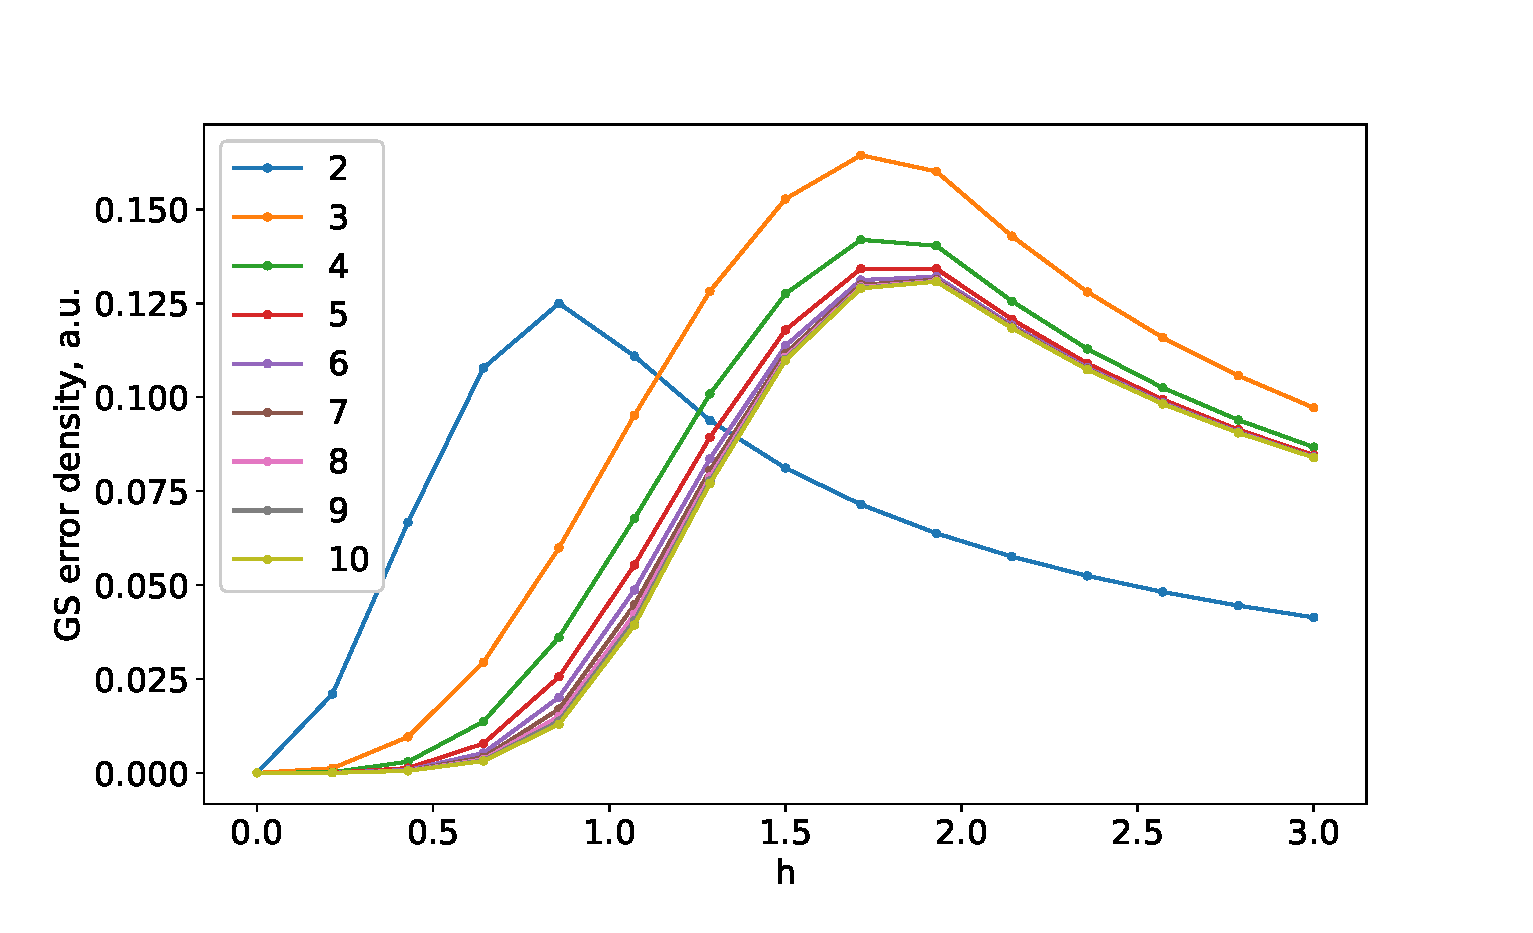
\includegraphics[width=0.7\textwidth]{figures/TFI_rank_one.eps}
    \caption{Error in ground state energy per qubit for ferromagnetic ($J = -1$) TFI model as a function of $h$. The approximate solutions are calculated using the unentangled ansatz state.}
    \label{fig:tfim_rank_one}
\end{figure}

\section{Variational quantum eigensolver}

\subsection{General description}

The variational principle inspired an algorithm for optimization of quantum Hamiltonians called variational quantum eigensolver (VQE). In short, we want to be able to estimate values like $\bra{\psi(\theta)} H \ket{\psi(\theta)}$ using a quantum computer. To do that, we need $\ket{\psi({\theta})}$ to be a state that can be prepared in the quantum processor (that is, a parametrized quantum circuit applied to some fixed reference state $\ket{\varphi}$), and $H$ needs to be an operator that acts in the space of qubits. 

Continuing the example of the spin model, we have a Hamiltonian consisting of $Z$ and $X$ operators. To do something about this model using a quantum computer, we identify each spin with a qubit (i.e.~for a spin chain with $n$ spins we need $n$ qubits). Since operators $Z$ and $X$ do not commute, they cannot be simultaneously measured. Hence, one has to measure them separately, in independent experiments. So, the subroutine for estimating $\bra{\psi(\theta)} H \ket{\psi(\theta)}$ is the following:

\begin{enumerate}
    \item Repeatedly prepare $\ket{\psi(\theta)}$ and measure each qubit in the standard basis. After enough measurements, estimate $\bra{\psi(\theta)} Z_i Z_{i+1} \ket{\psi(\theta)}$.
    \item Repeatedly prepare $\ket{\psi(\theta)}$ and measure each qubit in the $\{ \ket{+}, \ket{-} \}$ basis. After enough measurements, estimate $\bra{\psi(\theta)} X_i \ket{\psi(\theta)}$.
    \item Set $\bra{\psi(\theta)} H \ket{\psi(\theta)} := J \sum \bra{\psi(\theta)} Z_i Z_{i+1} \ket{\psi(\theta)} + h \sum \bra{\psi(\theta)} X_i \ket{\psi(\theta)}$.
\end{enumerate}

The trick here is that the qubits in the physical device do not have to have interactions prescribed by the model; all we need is to be able to prepare states and measure them in the standard basis (recall that measuring in the $\{ \ket{+}, \ket{-} \}$ basis is not much more difficult: we only need to apply a Hadamard gate to each qubit and then measure in the standard basis).

Now, assume that $\ket{\psi(\theta)}$ is a differentiable function of $\theta \in \mathbb{R}^k$ for some $k$, and $H \in \operatorname{Herm} (2^n)$. Then, the broad description of the VQE algorithm is the following loop:

\begin{enumerate}
    \item Estimate $E(\theta) = \bra{\psi(\theta)} H \ket{\psi(\theta)}$. 
    \item Use a classical optimization routine to find the next value of $\theta$. If the new value of $\theta$ is different from the old value by a threshold smaller than $\epsilon$, stop.
\end{enumerate}

A few remarks are in order:

\begin{itemize}
    \item In step 1, the estimate of $E(\theta)$ is sometimes replaced by the estimate of $\nabla E$, depending on the optimization routine in step 2. In the next subsection, we will give more detail the different choices of the optimization routine.
    \item The value $\bra{\psi(\theta)} H \ket{\psi(\theta)}$ is not easy to evaluate for any Hamiltonian. To be able to do that, we need to put additional restrictions on $H$. More precisely, we need $H$ to consist of a polynomial number of operators $h_i$ such that every expectation $\bra{\psi(\theta)} h_i \ket{\psi(\theta)}$ can be measured in polynomial time. An example of a Hamiltonian the conforms to this restriction is a Hamiltonian that consists of a polynomial number of Pauli strings. Alternatively, the Hamiltonian can consist of a polynomial number of projectors on product states.
\end{itemize}



\subsection{Optimization subroutine}

\paragraph{Stochastic graident descent.}
\textit{Gradient descent} is an algorithm of finding a local minimum of a differentiable function $f: \mathbb{R}^n \rightarrow \mathbb{R}$. The simplest variant of gradient descent goes as follows. Fix a \textit{learning rate} $\gamma > 0$ and pick an initial guess $x_0$. Then find the solution by repeating the following iteration:
\begin{equation}
    x_{i+1} = x_i - \gamma \nabla f(x_i).
\end{equation}
Stochastic gradient descent (SGD) appears when $\nabla f(x_i)$ is replaced by a random vector that estimates $\nabla f(x_i)$. In the context of supervised machine learning, stochastic gradient descent appears naturally: to calculate $\nabla f(x_i)$ exactly, one needs to iterate over all training samples, which is resource-intensive. Instead, the gradient is calculated over randomly chosen subsets of the training set called minibatches. The size of the minibatch seems to affect the quality of the solution. In paticular, there is evidence that with large batches SGD tends to find sharper minima that exhibit poorer generalization \cite{keskar_large-batch_2017}.

The learning rate $\gamma$ is also an important hyperparameter\footnote{A hyperparameter is a parameter of the model that is not updated during the training iterations, unlike e.g.~the weights of the neural network.} of the model. On the one hand, large learning rate means that the gradient descent may have trouble converging because large steps can overshoot the minimum. On the other hand, a small learning rate means more iterations. A simple change of the SGD that takes the best of both worlds consists in making $\gamma$ dependent on the iteration number, making it large in early steps and small in later steps. Of course, there are much more advanced variants of SGD with more complicated update rules, but reviewing them is outside the scope of this thesis. An interested reader can find the reviews of different SGD variants in Refs.~\cite{ruder_overview_2017,mehta_high-bias_2019}.

\paragraph{Gradient-free and gradient-based optimizers in VQAs.}

The optimization routines used for VQAs can be either gradient-based or gradient-free. Many experiments, both numerical and physical, used either class of methods for the optimization. Since there is no need to calculate gradient values in such mehtods, there is a reason to believe that they are more resilient to noise. Indeed, a naive implementation of gradient-based optimization would use finite differences to evaluate the gradient $\nabla E$:

\begin{equation}
    \label{eq:finite_difference}
    (\nabla E)_i = \frac{\partial E}{\partial \theta_i} \approx \frac{E(\theta_1, ..., \theta_i + \delta, ..., \theta_k) - E(\theta_1, ..., \theta_k)}{\delta}.
\end{equation}

However, this method is extremely unstable to the measurement errors. Indeed, if the variance of energy measurement is $\Delta$, then the variance of this difference is $\Delta^2 / \delta$. For this reason, many experimental implementations rely on gradient-free methods such as Nelder-Mead, Powell's method, or other techniques \cite{peruzzo_variational_2014,kokail_self-verifying_2019}. Another method used to mitigate the noisy measurements is to use the simultaneous perturbation stochastic algorithm (SPSA) \cite{spall_multivariate_1992} which evaluates the gradient by taking a finite-difference directional derivative in a random direction \cite{kandala_hardware-efficient_2017}. Despite even larger variance in the gradient, the appeal of this algorithm lies in the low cost of each individual iteration: for each step, the cost function needs to be evaluated just in two points. 

% \todo{A paragraph explaining some gradient-free optimization method, such as COBYLA or Nelder-Mead.}

As good as the gradient-free methods are, gradient-based optimization methods have better upper bounds on convergence. Ref.~\cite{harrow_low-depth_2019} adapts these bounds to the quantum variational aglorithms and introduces a gradient acquisition tehcnique based on the Hadamard test. Let the $H = \sum h_l \sigma_l$ be the Pauli decomposition of the cost function, and the ansatz be a product of unitaries whose generators also admit Pauli decompositions:
\begin{equation}
    \ket{\psi} = U_p ... U_1 \ket{\psi_0} = e^{-\rmi \frac{A_p \theta_p}{2}} ... e^{-\rmi \frac{A_1 \theta_1}{2}} \ket{\psi_0}; \quad A_j = \sum_{k=1}^{m_j} \beta_k Q_k.
\end{equation}
Then the partial derivative can be expressed as follows:
\begin{equation}
    \frac{\partial E}{\partial \theta_j} 
    = \sum_k \sum_l \beta_k h_l \operatorname{Im}
    \bra{\psi_0} 
    U_{1}^\dagger ... U_j^\dagger
    Q_k
    U_{j+1}^\dagger ... U_p^\dagger \sigma_l U_p ... U_1 \ket{\psi_0}.
\end{equation}
The imaginary value in the right-hand side can be evaluated from the output of the following circuit:
\begin{equation*}
    \Qcircuit @C=1em @R=1em {
    \lstick{\ket{+}} 
    & \qw 
    & \ctrl{1}
    & \qw
    & \ctrl{1}
    & \measureD{Y}
    \\
    \lstick{\ket{0...0}} 
    & \gate{U_j ... U_1} 
    & \gate{Q_k}
    & \gate{U_p ... U_{j+1}} 
    & \gate{\sigma_l}
    & \qw
    \\
    }
\end{equation*}

The variance of this measurement no longer has the dependence on a small step $\delta$ and is much more robust to experimental errors. However, the downside of that method is the requirement to implement $2n$ more control gates than in the ansatz circuit and that every partial derivative requires $m_j \operatorname{Card} H$ measurements.

Gradient-based methods became more prominent after the introduction of another estimation technique called parameter-shift rule \cite{mitarai_quantum_2018,schuld_evaluating_2019}. This rule is not harder to implement than the original ansatz circuit itself, at the cost of having to make more measurements. If the dependence on $\theta_i$ is realized as a quantum gate of the form $\exp(-\rmi G \theta_i/2)$, where $G$ has spectrum of $(-1, 1)$, then the exact value of the derivative can be obtained as follows:
\begin{equation}
    \label{eq:parameter_shift}
    \frac{\partial E}{\partial \theta_i} = \frac{1}{2} (E(\theta_1, ..., \theta_i + \pi/2, ..., \theta_k) - E(\theta_1, ..., \theta_i - \pi/2, ..., \theta_k)).
\end{equation}
To see why this is the case, let us consider the dependence of the ansatz on one variable $\theta$ while hiding all other unitaries in suitably redefined $\ket{\phi}$ or in $H$:
\begin{equation}
    E = \bra{\phi} e^{\rmi G \theta / 2} H e^{-\rmi G \theta / 2} \ket{\phi}.
\end{equation}
The partial derivative is then equal to 
\begin{equation}
    \frac{\partial E}{\partial \theta} = \bra{\phi} e^{\rmi G \theta / 2} \rmi F H e^{-\rmi G \theta / 2} \ket{\phi} - \bra{\phi} e^{\rmi G \theta / 2} \rmi HF e^{-\rmi G \theta / 2} \ket{\phi}.
\end{equation}
If we write down the values $E(\theta \pm \pi / 2)$ at shifted parameters, using the fact that $e^{\rmi G \pi / 4} = \frac{1}{\sqrt 2} (1 + \rmi G)$, we will get the desired formula by simple algebra.
The parameter-shift rule has been successfully used in VQAs \cite{sweke_stochastic_2019,barison_efficient_2021}, and recently it was generalized to the gates with arbitrary spectrum \cite{kyriienko_generalized_2021}.

The value of the gradient obtained in the experiment is a random variable that estimates the true value of $\frac{\partial E}{\partial \theta_i}$. Therefore, the optimization process is a random process itself, which means that formally the optimization process is an instance of stochastic gradient descent.

A good property of the abovementioned estimator is that it is unbiased, i.e.~the expected value of the estimate $\mathbb{E}\overline{\frac{\partial E}{\partial \theta_i}}$ is equal to the true value. However, its variance depends on the number of measurements made for the estimator. There is a question of efficiency: on the one hand, more measurements per step mean better estimation of the gradient, on the other hand, fewer measurements per step mean that the same budget of calls to the quantum device enables more steps of the gradient descent. What is then an optimal number of measurements per optimization step? This question was studied in Ref.~\cite{sweke_stochastic_2019}. The experiments of Sweke et al.~have shown that this number does not have to be large: in some of the tests, the optimal number of measurements per expected value per step is \textit{one}.



\subsection{Choice of the ansatz}

The ansatz $\ket{\psi(\theta)}$ can be constructed in a number of ways. Ignoring the variants of VQE which construct the ansatz iteratively (more on them later), the popular approaches are the problem-inspired ans\"atze and hardware-tailored ans\"atze.

\subsubsection{Problem-inspired ans\"atze}

A simple ansatz of that sort is called the Hamiltonian variational ansatz \cite{wecker_progress_2015}, which uses the operators comprising the target Hamiltonian as the generators for the quantum gates in the ansatz. For the transverse-field Ising model, such an ansatz could look like this:

\begin{equation}
    \ket{\psi(\theta)} = e^{i\theta_{2n} Z_n Z_1} ... e^{i\theta_{n+1} Z_1 Z_2} e^{i\theta_n X_n} ... e^{i\theta_1 X_1}\ket{\psi_0}.
\end{equation}

To increase the ``power'' of the ansatz (i.e.~the amount of states that it can prepare), this pattern of gates can be repeated. If we denote $U_{ZZ} (\xi_1, ..., \xi_n) = e^{i\xi_n Z_n Z_1} ... e^{i\xi_1 Z_1 Z_2}$, and $U_X(\xi_1, ..., \xi_n) = e^{i\xi_n X_n} ... e^{i\xi_1 X_1}$, then an $L$-layered Hamiltonian variational ansatz is as follows:
\begin{multline}
    \ket{\psi(\theta)} = 
    U_{ZZ} (\theta_{(2L-1)n+1}, ..., \theta_{2Ln})
    U_X (\theta_{(2L-2)n+1}, ..., \theta_{(2L-1)n})... \\
    ...
    U_{ZZ} (\theta_{n+1}, ..., \theta_{2n})
    U_X (\theta_1, ..., \theta_n) \ket{\psi_0}.
\end{multline}

% This ansatz is partially inspired by the quantum approximate optimization algorithm \cite{farhi_quantum_2014}, which in turn was inspired by quantum annealing. Hence, one can use the annealing schedule as an initial guess for the ansatz coefficients \cite{bosse_probing_2021}. \todo{They're probably not the first ones doing that. Find other references.}

Another popular problem-inspired ansatz, called the unitary coupled cluster \cite{taube_new_2006}, is used for quantum chemistry problems \cite{wecker_progress_2015,barkoutsos_quantum_2018,omalley_scalable_2016,shen_quantum_2017,xia_coupled_2020,xu_test_2020}. The ansatz is formulated in terms of the electronic structure problem and later translated to the language of qubits and circuits via different fermion-to-qubit-transforms. The problem is that fermionic operators obey the anticommutation relations, while no such relations are in place for qubits (i.e.~spins of distinguishable particles). In Section \ref{sec:fermion-transforms} we give an overview of such transforms.

The ansatz consists in approximately implementing a unitary operator comprising elementary electronic excitations:
\begin{equation}
\label{eq:ucc}
    \ket{\psi(\boldsymbol{\theta})} = 
    e^{T(\boldsymbol{\theta}) - T^\dagger(\boldsymbol{\theta})}
    \ket{\psi_0},
\end{equation}
where the operator $T$ is a sum of operators $T_1, ..., T_k$ corresponding to 1 to $k$ electronic transitions:
\begin{align}
    T_1 &= \sum_{i,j} \theta_{ij} a^\dagger_i a_j \\
    T_2 &= \sum_{i, j, k, l} \theta_{ijkl} 
    a^\dagger_i a^\dagger_j a_k a_l \\
    & ... \\
    T_k &= \sum_{i_1, ...,i_{2k}} \theta_{i_1 ... i_{2k}} 
    a^\dagger_{i_1} a^\dagger_{i_k} a_{i_{k+1}} ... a_{2k}.
\end{align}
The variational parameters are the real coefficients $\theta_{1_i ... i_m}$. Most often, the series of operators is truncated at $k = 2$, in which case the ansatz is called UCCSD (unitary coupled cluster, single and double).

There are certain difficulties with implementing this method on NISQ devices. The main trouble is that naive implementation of this ansatz leads to circuits whose depth is outside the reach of current NISQ hardware. Nonetheless, the UCC is a promising and actively studied subject (see \cite{anand_quantum_2022} for a review).

\subsubsection{Hardware-inspired ans\"atze}

One of the first things that one observes about the UCCSD ansatz is that its generic form is quite long. NISQ devices, however, prefer much shorter circuits. The variational principle works regardless of which ansatz you use, so one can try circuits that are coming from the restrictions of the hardware. 

One of the ans\"atze of that kind is now known as the hardware-efficient ansatz (HEA)\cite{kandala_hardware-efficient_2017}. The idea is simple: apply single-qubit gates to every qubit (this is easy), and then apply a sequence of entangling two-qubit gates.  Repeat this for a few rounds. What we obtain this way is a parametrized quantum circuit whose entangling power is adjusted by adding more layers. The two-qubit gates don't even have to be continuously parametrized, although they of course can be \cite{campos_abrupt_2020}. Typically, these are CNOT or CZ gates applied in a circular fashion to qubits $(i, i+1) \mod n$ (for example, see \cite{mcclean_barren_2018}). Sometimes the entangling gates are applied in an all-to-all fashion \cite{skolik_layerwise_2020}.

Another ansatz that is used for VQE is the so-called alternating layered ansatz, also known as the checkerboard ansatz \cite{uvarov_machine_2020,bravo-prieto_scaling_2020,cerezo_cost-function-dependent_2020}. This ansatz assumes line or ring connectivity of the qubits. Then it fixes some kind of two-qubit ansatz block and applies it in a checkerboard fashion: first, apply gates to qubit pairs $(2i, 2i+1)$, then, to pairs $(2i -1 , 2i)$. The block can be anything as long as it generates entanglement. For such circuits, it is easy to estimate the amount of entanglement generated across any bipartition using the theory of tensor networks and SVD \cite{biamonte_lectures_2020}. Another nice property is that, under some assumptions about the individual blocks, one can attempt to make some assertions about the whole circuit (moslty concerning its abitily to produce a random unitary operator \cite{brandao_local_2016}). The ansatz of that kind will be analyzed in depth in Chapter \ref{chap:plateaus}.



\section{Example: studying the electronic structure of a molecule}

In this section, we outline the whole procedure of applying VQE to a molecular Hamiltonian. We start with the nonrelativistic\footnote{In the second quantized picture though, the relativistic corrections end up having the same qualitative structure \cite{veis_relativistic_2012}.} Schr\"odinger equation for the electrons and nuclei of the molecule:

\begin{multline}
    H(\mathbf{r}_1, ..., \mathbf{r}_{N_e}, \mathbf{R}_1, ..., \mathbf{R}_{N_n}) = 
    \sum_{i=1}^{N_n} \frac{\hbar^2 \nabla^2}{2 M_i}
    + \sum_{i=1}^{N_e} \frac{\hbar^2 \nabla^2}{2 m_e} +\\
    + \sum_{i \neq j} \frac{Q_i Q_j}{|\mathbf{R}_i - \mathbf{R}_j|}
    + \sum_{i \neq j} \frac{1}{|\mathbf{r}_i - \mathbf{r}_j|}
    - \sum_{i=1}^{N_n} \sum_{j=1}^{N_e} \frac{Q_i}{|\mathbf{R}_i - \mathbf{r}_j|}.
\end{multline}

Since the mass of an electron is about $1/2000$'th of the mass of a proton, it is reasonable to introduce the Born--Oppenheimer approximation: for caluclation of the electronic structure, we consider the positions of the nuclei fixed, and the nuclei are treated as classical particles with potential interaction governed by the eigenstates of the electronic structure\footnote{This approximation is not always valid (for instance, if there is substantial coupling between electronic and vibrational degrees of freedom). For this situation, more advanced techniques are required \cite{yalouz_state-averaged_2021}.}.

Now, let's fix the nuclear positions $\mathbf{R}_i$ and only consider the electronic degrees of freedom. What we need to introduce now is the set of basis states $\psi_j(\mathbf{r})$. One could use the eigenstates of the hydrogen atom, but modern quantum chemistry provides us with a whole range of advanced basis sets. The one found most frequently in the VQE literature is the minimal STO-3G basis set: every state is a sum of three functions proportional to $x^i y^j z^k \exp(-\alpha (x^2 + y^2 + z^2))$. The word ``minimal'' means that there are as many basis states as there are atomic orbitals. More complex basis sets include more states than atomic orbitals (two per orbital, three per orbital, etc.) Such basis sets are called double-zeta, triple-zeta, and so on. In any case, such basis sets contain an infinite number of states, so we must limit ourselves to a finite subset. This truncation mainly depends on the number of qubits at our disposal.

Electrons cannot be together in the same state, so valid states of electrons are spanned by Slater determinants constructed out of single-electron states $\phi_i$ (also taking care of the spin degree of freedom $s_i$):

\begin{equation}
    \label{eq:slater}
    \Psi(\mathbf{r}_1, ..., \mathbf{r}_{N_e}, s_1,..., s_{N_e}) = \operatorname{det}
    \begin{pmatrix}
        \phi_1(\mathbf{r}_1, s_1) & ... & \phi_1(\mathbf{r}_{N_e}, s_{N_e}) \\
        ... & ... & ... \\
        \phi_{N_e}(\mathbf{r}_1, s_1) & ... & \phi_{N_e}(\mathbf{r}_{N_e}, s_{N_e}) \\
    \end{pmatrix}.
\end{equation}

Via Slater determinants, the basis set of single-electron functions induces a basis in the space of multi-electron wave functions called the Fock basis. The states in this basis can be denoted as $\ket{n_{0, \uparrow}, n_{0, \downarrow}, ...,  n_{k, \uparrow}, n_{k, \downarrow}, ...}$, where $n_{k, \uparrow}, n_{k, \uparrow} \in \{0, 1\}$ mark if the basis state is occupied. In the following, we will drop the spin degree of freedom from the notation and will treat the orbitals with different spin state as two distinct states. 

Now we need to rewrite the Hamiltonian in this basis. This is done using creation and annihilation operators. An \textit{annihilation operator} $a_i$ is defined as follows:
\begin{gather}
    \label{eq:fermi_annihilation}
    a_i \ket{n_1, ..., n_{i-1}, 0_i, ...} = 0; \\ 
    a_i \ket{n_1, ..., n_{i-1}, 1_i, ...} = (-1)^{n_1 + ... + n_{i-1}} 
    \ket{n_1, ..., n_{i-1}, 0_i, ...}.
\end{gather}
Its Hermitian conjugate $a^\dagger_i$ is called a \textit{creation operator}. Since the interactions we consider cannot create or destroy particles, these operators always come in pairs $a^\dagger_i a_j$, which means taking an electron from the site $j$ to the site $i$. Due to the fact that electrons are fermions, these creation-annihilation operators obey the following anticommutation relations: $\{a_i, a_j \} = 0, \{a_i, a^\dagger_j \} = \delta_{ij}$. 
% This idea of expressing multi-particle states in terms of population bases and creation-annihilation operators is known as second quantization and it can be found in many standard textbooks on quantum mechanics, e.g.~

The matrix elements of $H$ can be rewritten in terms of such operators as follows. For any pair of basis states, we can uniquely write down the combination of creation and annihilation operators that maps one state to the other (up to the ordering of the operators and excluding pairs like $a^\dagger_i a_i$), while mapping the other basis states to zero. This means that we can express any projector $\ket{\alpha} \bra{\beta}$ in such a form. The matrix elements $\bra{\Psi_i} H \ket{\Psi_j}$ are then calculated by integrating the respective wavefunctions over the three-dimensional space.

After calculating the coefficients and expressing everything in the secons quantized form, we arrive at the following Hamiltonian:
\begin{equation}
    H = \sum_{pq} h_{pq} a^\dagger_p a_q + \sum_{ijkl} V_{ijkl} a^\dagger_i a^\dagger_j a_k a_l.
\end{equation}
Observe that there are no terms of degree higher than four. The reason for that is the two-body nature of the Coulomb interaction. The matrix elements between Slater determinants consists of integrals of the form
\begin{equation}
    \int \phi^*_{m_1}(x_1) ... \phi^*_{m_k} (x_k) \frac{1}{x_i - x_j}
    \phi_{n_1}(x_1) ... \phi_{n_k} (x_k) dx_1 ... dx_k. 
\end{equation}
In such an integral, all terms not involving $x_i$ and $x_j$ can be integrated separately, while the orthonormality of the basis states ensures that the resulting factor is either zero or one, with the latter being the case when $m_l = n_l$. So any possible difference can only happen in positions $i$ and $j$.

Only a few steps remain for this Hamiltonian to become a problem accessible to VQE. First, we assume that some of the low-lying states are always occupied, and that the states that are higher than a certain energy threshold are always empty. The space of states that we keep considering is called the \textit{active space}. The larger that space is, the better is the quality of the approximation. Finally, we need to identify electronic orbitals with qubits by using either the Jordan--Wigner or Bravyi--Kitaev transformation (Section \ref{sec:fermion-transforms}). Now the problem is completely ready for solution via VQE. We choose the ansatz, the optimization method, and run the algorithm.

\section{Fermion-to-qubit transformations}
\label{sec:fermion-transforms}

Fermionic operators are described in terms of creation and annihilation operators. Due to the permutation antisymmetry of fermionic wavefunctions, these operators obey peculiar anticommutation relations: $\{a_i, a^\dagger_j\} = \delta_{ij}, \{a_i, a_j\} = 0$. Qubits, on the other hand, are distinguishable particles. A mapping from fermions to qubits must respect these relations. Below are a few different methods to achieve that. In this section, we follow the original work \cite{bravyi_fermionic_2002} and the detailed exposition of \cite{seeley_bravyi-kitaev_2012}.

\subsection{Jordan--Wigner transform}

The simplest way to map fermions to qubits is to identify each qubit with a fermionic mode. To preserve the relations, an annihilation operator $a_i$ is mapped to an operator acting on qubit $i$, times a trail of operators counting the parity of the population of the preceding modes:
\begin{equation}
    a_i \mapsto f_i := Z_1 ... Z_{i-1} \otimes 
    \begin{pmatrix}
        0 & 1 \\
        0 & 0 \\
    \end{pmatrix} = Z_1 ... Z_{i-1} (X_i + \rmi Y_i) / 2.
\end{equation}
Comparing this with Eq. (\ref{eq:fermi_annihilation}), we can see that $f_i$ acts on the qubit registry exactly like $a_i$ acts on fermions.


\subsection{Bravyi--Kitaev transform}

The Bravyi--Kitaev transform \cite{bravyi_fermionic_2002} maps $m$ fermions to $m$ qubits by storing the parity information in a more elaborate way. The idea is to encode both the population information and parity information in a way that would require a logarithmic number of qubits to calculate.

Denote an $m$-site fermion state $\ket{n_0, ..., n_{m-1}}$ and the corresponding $m$-qubit state $\ket{x_0} \ket{x_2} ... \ket{x_{m-1}}$ 
% (note that we start counting the registers from one, unlike the notation in \cite{bravyi_fermionic_2002,seeley_bravyi-kitaev_2012}; the reason for that change will be clear in a moment). 
To encode one state into the other means to provide a function that maps $(n_0, ..., n_{m-1})$ to $(x_0, ..., x_{m-1})$. Bravyi and Kitaev provide the following function:
\begin{equation}
    \label{eq:bk_formula}
    x_j = n_j + \sum_{s \prec j} n_s \ (\operatorname{mod} 2),
\end{equation}
where the partial order $\prec$ is introduced on as follows. Two numbers are written in their binary expansions $\alpha_{t-1} ... \alpha_0$, $\beta_{t-1} ... \beta_{0}$. We say that $\alpha_{t-1} ... \alpha_0 \preceq \beta_{t-1} ... \beta_{0}$ if there is a position $l_0$ such that (1) $\beta_l = 1 \ \forall l < l_0$ and (2) $\alpha_l = \beta_l \ \forall l \geq l_0$. That is, if the binary expansions of $a$ and $b$ match up to a certain position, and all lower positions of $b$ are equal to one, then $a \preceq b$.

For example, if we expand (\ref{eq:bk_formula}) as a matrix-vector equation over $\mathbb{F}_2$ for the example of $m = 8$, we will get the following (zeros are written as blank spaces for visual clarity):

\begin{equation}
    \label{eq:bk_matrix}
    \begin{pmatrix}
        x_0 \\ x_1 \\ x_2 \\ x_3 \\ x_4 \\
        x_5 \\ x_6 \\ x_7 \\
    \end{pmatrix} = 
    \begin{pmatrix}
    1 &   &   &   &   &   &   &   \\   
    1 & 1 &   &   &   &   &   &   \\
      &   & 1 &   &   &   &   &   \\
    1 & 1 & 1 & 1 &   &   &   &   \\
      &   &   &   & 1 &   &   &   \\
      &   &   &   & 1 & 1 &   &   \\
      &   &   &   &   &   & 1 &   \\
    1 & 1 & 1 & 1 & 1 & 1 & 1 & 1 \\
    \end{pmatrix} 
    \begin{pmatrix}
        n_0 \\ n_1 \\ n_2 \\ n_3 \\ n_4 \\
        n_5 \\ n_6 \\ n_7 \\
    \end{pmatrix} 
    .
\end{equation}
This is somewhat opaque, but observe the following. If we need to know the parity of $a_j$, i.e.~$P_j := n_0 + ... + n_{j-1}$, we need to sum up the $x_k$ such that $k+1$ is obtained by taking the expansion of $j$ in the powers of two and throwing away several lowest terms. For example, $P_7 = x_6 + x_5 + x_3$, and $P_6 = x_5 + x_3$. In any case, the parity information is stored in no more than $\log_2 m$ qubits\footnote{Also observe that the matrix in (\ref{eq:bk_matrix}) looks somewhat like the Sierpi\'nski triangle.}. For each $j$, we will denote as $P(j)$ the set of qubits that is required to find the parity.

Next, we need to find qubits which contain $n_j$. Again, by construction of the sets $S(j)$ there is a logarithmic number of such qubits. We will denote this set $U(j)$.

The application of $j$ depends on whether it is odd or even. For $j$ even, $a_j$ maps to the following operator:
\begin{equation}
    \label{eq:aj_bk_even}
    a_j \mapsto \left(\bigotimes_{i \in P(j)} Z_i\right) \otimes \left(\bigotimes_{k \in U(j)} X_k \right) \otimes 
    \begin{pmatrix}
    0 & 1 \\
    0 & 0 \\    
    \end{pmatrix}_j.
\end{equation}
For $j$ odd, the calculation is somewhat more involved. The reason for this is that, for $j$ even, the mapping is very simple: $x_j = n_j$. For $j$ odd, it is somewhat more laborious to account for the population $n_j$ correctly. Denote $F(j)$ the set of qubits that have the same parity as the orbital $j$. Then define an operator $\Pi_j$ as
\begin{equation}
    \Pi^-_j = \frac12 \left(X_j \otimes \bigotimes_{i \in F(j)} Z_i + \rmi Y_j\right).
\end{equation}
Finally, for $j$ odd, the annihilation operator maps to:
\begin{equation}
    \label{eq:aj_bk_odd}
    a_j \mapsto \left(\bigotimes_{i \in P(j) \backslash F(j)} Z_i\right) \otimes \left(\bigotimes_{k \in U(j)} X_k \right) \otimes 
    \Pi^-_j.
\end{equation}
The creation operator $a^\dagger_j$ can be obtained from Eqs.\,(\ref{eq:aj_bk_even}, \ref{eq:aj_bk_odd}) by taking the usual Hermitian conjugate. The sizes of $P(j)$ and $U(j)$ are logarithmic in $m$, so the operators will have logarithmic locality.

\section{Potential applications of VQE}

\subsection{Quantum chemistry}
%todo group by something, maybe not around test models
The most prominent application of VQE so far is quantum chemistry. Indeed, many proof-of-concept experiments \cite{peruzzo_variational_2014,omalley_scalable_2016,kandala_hardware-efficient_2017,hempel_quantum_2018,shen_quantum_2017}, as well as numerical simulations \cite{parrish_quantum_2019,romero_strategies_2017}, consider small molecules as target Hamiltonians. In the Born--Oppenheimer approximation, VQE returns the energy of the electronic ground state for the specific locations of the nuclei. Solving the same problem for different positions provides an energy landscape for the interaction of the nuclei. This way, one could potentially learn the pathways taken by molecules during chemical reactions. To do that, one needs to resolve the energy level up to \textit{chemical accuracy}, which is typically considered to be 1 kcal/mole. Since the chemical reactions often involve going over potential barriers, the rates of reactions are exponentially sensitive to the height of said barriers and hence to the error of the computation. To do well, we need to include many energy levels, whcih may lead to unfavorable scaling of simulation time just because of the sheer number of parameters to be optimized in a generic ansatz \cite{elfving_how_2020}. Nonetheless, advanced techniques in designing the VQE experiment --- discussed in the next section --- may prove useful in dealing with this problem.

\subsection{Condensed matter physics and lattice QFT}

One can apply VQE to lattice electronic problems (e.g.~Hubbard model) in a rather straightforward way \cite{cade_strategies_2019,uvarov_variational_2020}. The approach is the same as for the chemical Hamiltonians, except that instead of orbitals, the basis single-electron states are the lattice sites. Then one can proceed with Bravyi--Kitaev or Jordan--Wigner transformation.

In an experiment in \cite{kokail_self-verifying_2019}, the authors apply VQE to a model derived from lattice quantum field theory. Each site of a lattice can contain either an electron, or a positron, or both. For that reason, every lattice site is in fact simulated by two lattice sites: even-numbered sites are populated with electrons, while odd-numbered sites are populated with positrons. Other than that, the mapping to qubits is mostly the usual Jordan--Wigner transform.

There is also an alternative approach to variational investigation of quantum systems which involves variational calculation of the Green's function of the system~\cite{endo_calculation_2020}.

\subsection{Classical optimization problems}

Classical optimization problems can be embedded into quantum Hamiltonians to be then solved via VQE. For example, it is easy to embed the problem called \textsc{MaxCut}. Since this problem is \textbf{NP}-complete, this already enables the solution of many other classical problems.

The problem is formulated as follows. Let $G = (V, E)$ be an undirected graph. A \textit{cut} is a partition of the vertex set $V$ into two subsets. The \textit{size of the cut} is defined to be the number of edges connecting vertices from different subsets. In other words, if we group the vertices in two piles, the size of the cut is the number of edges connecting the two piles. The task is to find the maximum cut. 

This task can be expressed as a Hamiltonian minimization problem as follows. identify a qubit with each vertex, with $\ket{0}$ and $\ket{1}$ being the labels of this vertex belonging to piles one and two, respectively. For every edge $(i, j) \in E$, we would like to introduce a penalty if the edge is not cut. This can be done by a term $Z_i Z_j$. Summing up over the edges, we end up with an antiferromagnetic Ising model defined on the graph $G$:

\begin{equation}
    \label{eq:maxcut_ising}
    H = \sum_{(i, j) \in E} Z_i Z_j.
\end{equation}

This embedding of classical problems into VQE is related to the idea of continuous relaxation of problems [McClean low-depth 2021]. In particular, the analogy is quite vivid if the ansatz is a very simplistic one that doesn't introduce entanglement \cite{bittel_training_2021}. 

Continuous relaxation means the following: instead of $\{-1, 1\}$, the vertices are assigned points on a high-dimensional sphere. The solution to the continuous problem (in case of MaxCut) can be found by means of semidefinite programming. This solution is then mapped back to the discrete solution by simply cutting the sphere into random halves. For MaxCut, this approach is known as the Goemans--Williamson algorithm. Under certain plausible assumptions, it is $\mathbf{NP}$-hard to solve MaxCut with a better approximation ratio than with this algorithm.

At current state it seems that the outlook of VQE for classical problems is not very promising: entanglement-free ans\"atze can be simulated without a quantum computer, and simple entangled ans\"atze, at least in a numerical experiment in Ref.~\cite{nannicini_performance_2019}, do not seem to yield any substantial improvement in optimization results. The quantum approximate optimization algorithm (QAOA, see Section~\ref{sec:vqa_related}), which is a variant of VQE with a peculiar ansatz, is also actively investigated as a tool to solve classical problems.

\section{Variants of VQE}
\label{sec:vqe_variants}

The basic variant of VQE is quite generic. It of course invites many different modifications. Here we will survey some of the prominent proposals.

\subsection{Variants that modify the cost function}

\paragraph{Adiabatically-assisted VQE.} Since the optimization version of the \textsc{local Hamiltonian} problem is $\mathbf{QMA}$-hard, one could expect that the optimization landscape is very nonconvex, and convergence to suboptimal minima is a very possible thing. To counter this, Ref.~\cite{garcia-saez_addressing_2018} borrows an idea from adiabatic quantum computing. Let $H$ be the problem Hamiltonian and $H_{\text{init}}$ some Hamiltonian whose ground state is easy to prepare. Denote $H_s = (1-s)H_{\text{init}} + sH$. Find the ground state of $H_0$, and then run VQE for each $H_{s + \Delta s}$, using the solution of $H_{s}$ as a starting point. This may look very inefficient, since now you have to solve many VQE problems instead of one, but these intermediate problems may converge much faster because the starting point is already close to an exact solution. In Chapter \ref{chap:vqe_numerics}, we adopt this variant to solve the ground state problem for the transverse-field Ising model at different field strengths.

\paragraph{Meta-VQE.} Recall that when we discussed quantum chemistry, we introduced the Born-Oppenheimer approximation that essentially decouples the electronic motion and the nuclear motion. In order to predict chemical reactions and coupling energies, one needs to find e.g.~optimal distances between atoms. This implies that one has to solve many similar VQE problems for different values nuclei positions $\{\mathbf{R}_i\}$. To do this, Meta-VQE lets some parameters of the ansatz be functions of the nuclei positions. This way, when the ansatz is optimized, it gives some approximation to all problems simultaneously. This approximation is far from chemical precision, but it provides a good inital point for further VQE solution of individual problems, which quite important in the view of the barren plateaus phenomenon discussed in Chapter~\ref{chap:plateaus}.

\paragraph{Divide-and-conquer.} Ref.~\cite{fujii_deep_2020} proposes a variant of VQE --- dubbed Deep VQE --- that is reminiscent of the famous DMRG method. In Deep VQE, the quantum system is split into several subsystems. The Hamiltonian is then naturally separated into local terms and subsystem-subsystem interaction terms. The algorithm runs VQE for each subsystem separately, finding the ground states and a number of low-energy exctitations. Then the interaction terms are projected to the low-energy subspaces of the subsystems. Finally, this new problem is mapped to qubits and solved again via VQE. As a result, the solution is found using a smaller number of qubits, possibly at a cost of increased energy error.

\subsection{Variants that dynamically update the ansatz structure}

\paragraph{Adapt-VQE.} Optimizing large circuits requires many estimations of derivatives, that is why it is a good idea to start with a small ansatz and increase it along the way. This is the idea of Adapt-VQE \cite{grimsley_adaptive_2019}: first, one fixes some pool of Hermitian operators $F_i$ that one wishes to use in the ansatz. For chemical problems, such operators are one- and two-particle excitations. Then, for each operator in the pool, one can estimate the derivative that one would get if one appended a parametrized gate $\exp{\mathrm{i} \theta F_i}$ to the end of the circuit. The gate with the largest derivative (by magnitude) is then chosen and appended to the ansatz. Optimize over the ansatz parameters and repeat. For small molecules, this seems to provide better results than the UCCSD ansatz while using fewer gates. 

Some modifications of this algorithm were proposed in the literature. One is qubit-adapt-VQE \cite{tang_qubit-adapt-vqe_2021}, which replaces fermionic excitations by two-qubit Pauli operators, and batched adapt-VQE \cite{sapova_variational_2021}, which adds more than one generator per iteration.

\paragraph{Ansatz pruning.} This idea was independently explored in \cite{bilkis_semi-agnostic_2021} and \cite{sim_adaptive_2021}. After constructing the ansatz, one can find that some gates are close to the identity. Such gates can often be eliminated without affecting the quality of the solution too much. This procedure can be combined with iterative ansatz growing techniques like ADAPT-VQE.

\paragraph{Genetic evolution of ans\"atze.} Ref.~\cite{chivilikhin_mog-vqe_2020} proposes updating the ansatz with a genetic algorithm. Genetic algorithms are inspired by evolution of species in nature: a pool of candidate solutions is sorted according to the fitness score (energy obtained by minimization plus a penalty depending on the depth of the circuit). The next generation of candidate solutions is produced by combining the successful solutions (this is done by a crossover of two circuits: two lists of gates are split at a random point, then the head of one is concatenated with the tail of the other and vice versa) and introducing mutations in the form of randomly inserted/removed gates. The proposed algorithm optimizes both for the energy of the solution and for the number of gates in the ansatz circuit.

\subsection{Other}

\paragraph{Quantum subspace expansion.} Suppose after optimizing over the problem Hamiltonian $H$, the algorithm came up with a state $\ket{\psi}$. Then quantum the subspace expansion (QSE) algorithm \cite{mcclean_hybrid_2017,colless_computation_2018} gives a prescription on how to evaluate not only the energy $\bra{\psi} H \ket{\psi}$, but also values of the kind $\bra{\psi_i} H \ket{\psi_j}$ for some closely-related states $\ket{\psi_i}$. The idea is that, if $\sigma_i$ and $\sigma_j$ are some Pauli strings, then the Pauli decomposition of $\sigma_i H \sigma_j$ has the same cardinality as the Pauli decomposition of $H$. This means that the value can $\bra{\psi} \sigma_i H \sigma_j \ket{\psi}$ can be estimated by a standard procedure. Physically the operators $\sigma_i$ are meant to mimic some few-particle excitation operators, which means that the states $\ket{\psi_i}$ should not be too far in energy from the state $\ket{\psi}$. In any case, after this procedure we can build the matrix elements of $H$ projected onto the subspace spanned by $\ket{\psi_i}$ and diagonalize it classically. This may improve the energy estimate of the ground state and also provide estimations of the energies of low-lying excited states.

A related proposal is described in Ref.~\cite{bharti_iterative_2020}. This algorithm also approximates the ground state of a target Hamiltonian, but does so by taking inner products of candidate states. Essentially, it runs the quantum subspace expansion for a fixed input state, then takes second-order perturbations by taking products of two Pauli strings, and so on until the desired precision is reached.

\paragraph{Qubit coupled cluster.} In VQAs, there is heavy use for alternating between the Schr\"odinger picture of quantum mechanics and the Heisenberg picture. In the latter, the quantum state is fixed, and quantum evolution acts by conjugation on the observables. The approach suggested in Refs. \cite{ryabinkin_iterative_2020,ryabinkin_qubit_2018} exploits the Heisenberg picture by applying some generators of the ansatz directly to the target Hamiltonian instead of the quantum state. At the cost of increased Hamiltonian cardinality, this method may potentially simplify the ansatz state, making it better suited for running on NISQ devices.

\section{Related algorithms}
\label{sec:vqa_related}


\subsection{Quantum neural network training}

An interesting direction of research lies at the intersection of variational quantum algorithms and machine learning. A parametrized quatnum circuit can be treated as a device that accepts a quantum state and returns a probability distribution of measurements. One can use this approach to solve a classification problem for quantum states. This is covered in more detail in Chapter \ref{chap:qml}.

\subsection{QAOA}

Quantum-assisted optimization algorithm (QAOA) \cite{farhi_quantum_2014} is an algorithm that can be considered a variant of VQE with a fixed ansatz structure. Let $H_0$ be the Hamiltonian of an easy problem, and let $H$ be the problem of interest. Then the QAOA ansatz is the alternating sequence of evolution operators\footnote{Later on, this circuit structure became known as ``Quantum alternating operator ansatz'', the acronym being the same as before.} generated by $H_0$ and $H$, acting on the ground state of $H_0$:

\begin{equation}
    \ket{\psi(\gamma_1, ..., \gamma_p, \beta_1, ..., \beta_p)}
    = e^{-\rmi \beta_p H_0} e^{-\rmi \gamma_p H} ... e^{-\rmi \beta_1 H_0} e^{-\rmi \gamma_1 H} \ket{\psi_0}.
\end{equation}

In practice, the Hamiltonian $H_0$ is taken to be the sum of single-qubit $X$ operators: $H_0 = \sum X_i$. Its ground state is the product of plus states $\ket{+}^{\otimes n}$. The initial proposals and investigations considered QAOA for classical optimization problems like MaxCut \cite{farhi_quantum_2017}, but later on it was also used for optimal preparation of quantum gates \cite{kiani_learning_2020} and Hamiltonian minimization \cite{ho_efficient_2019}.

\subsection{Optimized preparation of quantum gates}

While VQE finds an optimal state, one can also adopt the variational paradigm to the task of finding a circuit preparing a desired gate. This algorithm is called variational quantum gate optimization (VQGO) \cite{heya_variational_2018}. The variational circuit $U(\boldsymbol{\theta})$ is optimized to maximize the fidelity between the experimental output $U(\boldsymbol{\theta}) \rho U^\dagger (\boldsymbol{\theta})$ and the (simulated) output $U_\text{ideal} \rho U^\dagger_\text{ideal}$, averaged over random input states $\rho$.

An alternative algorithm for the similar task is known as quantum-assisted quantum compiling \cite{khatri_quantum-assisted_2019}. This algorithm uses two quantum registers. First, all qubits of these registers are coupled in Bell pairs ($i$'th qubit of register A to $i$'th qubit of register B). Then, a fixed gate $U$ is prepared in the first register, and a variational circuit $V^*$ is prepared in the second register. By measuring in the Bell basis, one can evaluate $|\Tr UV^\dagger|^2$ and optimize it with a classical computer. As a result, the conjugate $V$ will be as close to $U$ as possble. Naturally, there is a question: if we can already prepare a gate $U$, why bother with trying to make its copy with a variational ansatz? There are several propositions. First, one can try to compress quantum circuits this way. Second, if $U$ is implemented by an unknown process, one can recover a circuit describing this process. Finally, if the qubits in different registers have different quality, this procedure can be used for comparison or for noise correction.

\subsection{Variational state preparation}

Variational approach can be used to optimize the preparation of a state described by a known quantum circuit. A way to do that is described in \cite{biamonte_universal_2021}. The idea is to construct a cost function that is minimized by the target state and run VQE against that cost function. One such cost function is a the so-called telescope construction. It is simple, but its downside is that its cardinality grows exponentially with the number of non-Clifford gates. Another construction is already known as the Kitaev clock construction \cite{kitaev_classical_2002}. 

% \subsection{Iterative quantum-assisted eigensolver}




% \section{Numerical results} \label{sec:vqe_numerics}
% \subsection{TFI and XXZ Heisenberg models}

% \subsection{Training a quantum classifier of VQE data}

% \subsection{Hubbard model with next-nearest-neighbor repulsion}

% We also had some plots with pop vs chemical potential, they can go here.

\section{VQE vs. phase estimation algorithm}

Variational quantum eigensolver is not the first quantum algorithm proposed for solution of hard optimization problems. An earlier proposal is known as the phase estimation algorithm (PEA). This algorithm is based on the quantum Fourier transform and the ability to make a controlled execution of $U = \exp(\mathrm{i} \tau H)$.

PEA works as follows. Prepare an approximate ground state $\ket{\psi}$ in one register, and the plus state $\ket{+}^{\otimes m}$ in an $m$-qubit ancilla register. 

Then apply $U$ controlled on the first qubit, $U^2$ controlled onthe second qubit, $U^4$ controlled on the third qubit, and so on, doubling the power for each qubit. The register with $\psi$ will remain unentangled with the control register. If $\ket{\psi}$ is an eigenstate of $U$ with $U\ket{\psi}=e^{2\pi \rmi \phi}$, the control register will now have the Fourier transform of $\phi$. Inverse FT yields the answer.

If $\ket{\psi}$ is not an eigenstate of $H$, then we'll have a superposition of states. Let $U = e^{i \tau H}$, and $|\psi \rangle = \sum c_i | \lambda_i \rangle$. Then after PEA we will obtain a state $| \phi \rangle = \sum c_i (e^{i \tau \lambda_i} |\lambda_i \rangle \otimes |\text{QFT}_i \rangle)$. Then with probability $|c_i|^2$, we will obtain the necessary eigenvalue.

Solution of the ground state problem using PEA has been experimentally demonstrated a number of times \cite{whitfield_ground_2012,lanyon_towards_2010,bauer_hybrid_2016,omalley_scalable_2016}. Compared to VQE, this algorithm has an advantage that the number of runs required to find the ground state energy to precision $\epsilon$ is estimated as $O(\epsilon^{-1})$, whereas for VQE the evaluation of energy \textit{in each iteration} is about $O(\epsilon^{-2})$ (however, one doesn't necessarily have to obtain such precision in each iteration: the paper \cite{sweke_stochastic_2019} argues evaluation of derivatives in small experimental samples is also a viable strategy; nonetheless, the final answer has to be evaluated to good precision). 

The downsides are the complexity of the required quantum circuit and the requirement that the initial state has significant overlap with the true ground state. The latter is sometimes referred to as ``orthogonality catastrophe'' \cite{kohn_nobel_1999}. While complexity-theoretical intuition suggests that this catastrophe cannot be avoided completely --- otherwise we would be able to solve $\mathbf{QMA}$-complete problems in quantum polynomial time --- some remedies for practical problems are investigated in the literature \cite{tubman_postponing_2018}.

Even with the better asymptotic scaling, PEA may still be quite computationally expensive for practical problems. Ref.~\cite{reiher_elucidating_2017} estimates the resource requirement for calculating the chemical reactions involving the so-called iron-molybdenum cofactor (FeMoco). This molecule is a critical element of the enzyme that takes part in biological nitrogen fixation, i.e.~the process of transforming atmospheric nitrogen into ammonia. Reiher et al.~conclude that the resources required for simulating FeMoco are comparable to those required for factoring 4096-bit integers using the Shor's algorithm. Will VQE fare even worse? Who knows.

The comparison of these algorithms makes some authors suggest that VQE is an algorithm for noisy devices with low available depth, and in the era of fault-tolerant, large-scale QCs it may be gradually replaced by PEA \cite{elfving_how_2020}. In the meantime, there is a proposal to combine the two approaches by using both kinds of measurements in a varying proportion \cite{wang_accelerated_2019}.